% Set up the document class - this can be changed if a different format is required 
\documentclass[11pt,a4paper,oneside]{article}

% Include packages that contain additional features, for example including special mathematical characters and images in your document
\usepackage{amssymb,amsmath,graphicx}
\usepackage[T1]{fontenc} 
\usepackage[utf8]{inputenc}   % here are our umlauts...
\usepackage{graphicx} % ...and our graphics

\usepackage{bold-extra}
\usepackage[plainpages=false, pdfpagelabels, colorlinks=true, breaklinks=true, linkcolor=black, menucolor=black, urlcolor=black, citecolor=black]{hyperref}
\usepackage[font=sf, labelfont={sf,bf}, margin=1cm]{caption}
\usepackage[b]{esvect}
% Long equations
\usepackage{breqn} 
%include pdfs
\usepackage{pdfpages}
\usepackage{hyperref}
\usepackage{epstopdf}
%\usepackage{fullpage}
\usepackage{placeins}

\usepackage{listings}
\lstloadlanguages{Python} % Load python syntax for listings, for a list of other languages supported see: ftp://ftp.tex.ac.uk/tex-archive/macros/latex/contrib/listings/listings.pdf
\DeclareFixedFont{\ttb}{T1}{txtt}{bx}{n}{9} % for bold
\DeclareFixedFont{\ttm}{T1}{txtt}{m}{n}{9}  % for normal
\usepackage{color}
\definecolor{deepblue}{rgb}{0,0,0.5}
\definecolor{deepred}{rgb}{0.6,0,0}
\definecolor{deepgreen}{rgb}{0,0.5,0}


% The beginning of the document...
\begin{document}
% configure standard code listings:
\lstset {
	language=Python,
	backgroundcolor=\color{white}, %%%%%%%
	basicstyle=\ttm,
	otherkeywords={self},            
	keywordstyle=\ttb\color{deepblue},
	emph={MyClass,__init__},          
	emphstyle=\ttb\color{deepred},    
	stringstyle=\color{deepgreen},
	commentstyle=\color{red},  %%%%%%%%
	frame=tb,                         
	showstringspaces=false,
	numbers=left
}

\renewcommand\thesubsection{\alph{subsection})}

% Please change the following accordingly...
\centerline{\LARGE \textbf{Artificial Intelligence - Exercise Sheet 9}}\vspace{0.5em}
\centerline{\large by Lucas-Raphael Müller}\vspace{2em}


\section{Variants of SGD}
Given an objective function, which is a function of the parameters $\theta$ and the samples ${x_i}$, $Q$ is often of the following form:
\begin{equation}
	Q = Q(\theta, x) = \sum\limits_i Q_i(\theta, x_i).
\end{equation}
\paragraph{Batch Gradient Descent} Gradient descent would now mean
\begin{equation}
	\theta := \theta - \eta \nabla Q(\theta, x),
\end{equation}
with $\eta$ for the learning rate.

\paragraph{Stochastic Gradient Descent} Instead of iterating over all samples (i.e. computing the sum), stochastic gradient descent uses just a single sample and estimates the gradient.
Therefore, stochastic gradient descent is much faster.

\paragraph{Mini-Batch Gradient Descent} In mini-batch gradient descent a (small) subset of the whole training dataset $x$ is being used as a compromise between batch and stochastic gradient descent, and performance vs. speed.

\section{Implementing an Autoencoder}
I was unsure, how the first linear layer was actually meant. So whether it was input layer plus linear layer of again 8 neurons, or just the input layer (line 56, as above).
I also saw no point in just reporting every 10th epoche for testing, since testing is performed once per epoch?

Implemented autoencoder as follows:
\lstinputlisting[language=Python]{autoencoder.py}

\begin{figure}
	\centering
	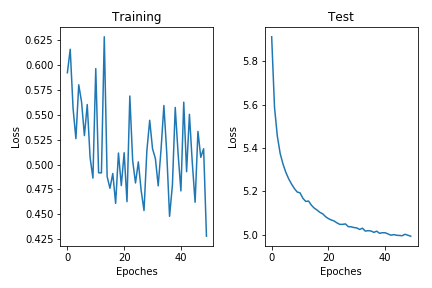
\includegraphics[width=.9\textwidth]{figures/auto_encoder_evolution}
	\caption{Evolution of Train and Test loss.}
\end{figure}
\begin{figure}[!btp]
	\centering
	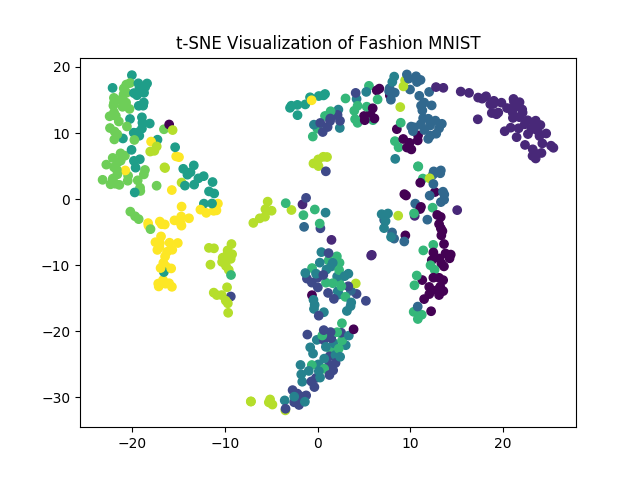
\includegraphics[width=.9\textwidth]{figures/t_sne}
	\caption{TSNE representation.}
\end{figure}
\begin{figure}[!btp]
	\centering
	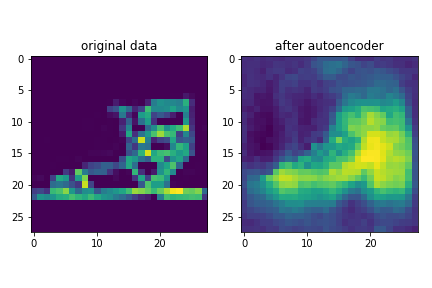
\includegraphics[width=\textwidth]{figures/save_ev_0}
	\caption{Original Image and after autoencoder.}
\end{figure}
\begin{figure}[!btp]
	\centering
	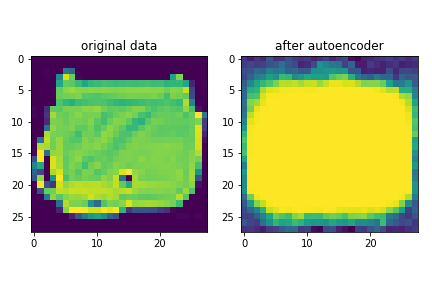
\includegraphics[width=\textwidth]{figures/save_ev_1}
	\caption{Original Image and after autoencoder.}
\end{figure}
\begin{figure}[!btp]
	\centering
	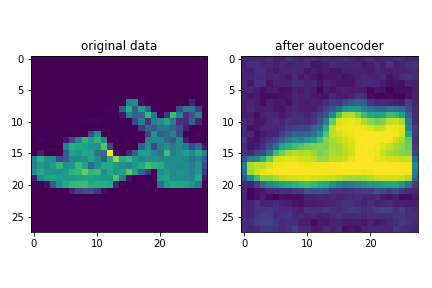
\includegraphics[width=\textwidth]{figures/save_ev_2}
	\caption{Original Image and after autoencoder.}
\end{figure}
\begin{figure}[!btp]
	\centering
	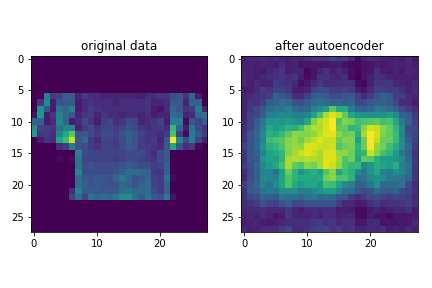
\includegraphics[width=\textwidth]{figures/save_ev_3}
	\caption{Original Image and after autoencoder.}
\end{figure}
\begin{figure}[!btp]
	\centering
	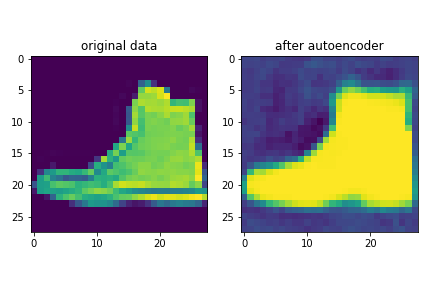
\includegraphics[width=\textwidth]{figures/save_ev_4}
	\caption{Original Image and after autoencoder.}
\end{figure}
\begin{figure}[!btp]
	\centering
	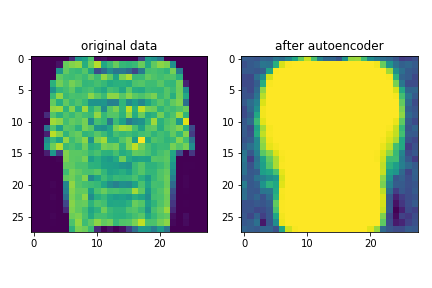
\includegraphics[width=\textwidth]{figures/save_ev_5}
	\caption{Original Image and after autoencoder.}
\end{figure}
\begin{figure}[!btp]
	\centering
	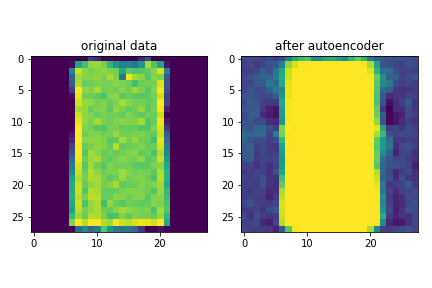
\includegraphics[width=\textwidth]{figures/save_ev_6}
	\caption{Original Image and after autoencoder.}
\end{figure}
\begin{figure}[!btp]
	\centering
	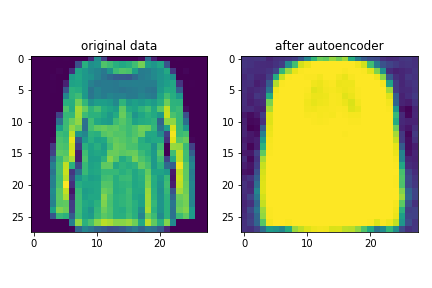
\includegraphics[width=\textwidth]{figures/save_ev_7}
	\caption{Original Image and after autoencoder.}
\end{figure}
\begin{figure}[!btp]
	\centering
	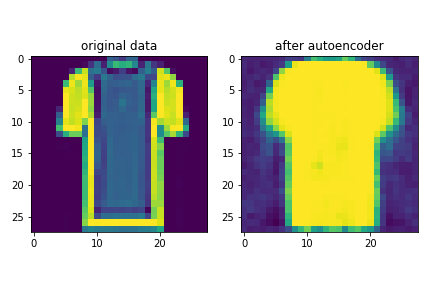
\includegraphics[width=\textwidth]{figures/save_ev_8}
	\caption{Original Image and after autoencoder.}
\end{figure}
\begin{figure}[!btp]
	\centering
	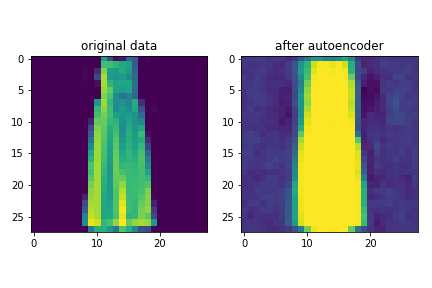
\includegraphics[width=\textwidth]{figures/save_ev_9}
	\caption{Original Image and after autoencoder.}
\end{figure}

\FloatBarrier
\section{Denoising Autoencoder}
I could not see much of a difference between both autoencoders. 
This is probably because noise does not alter principal components (important eigenvalues).
\begin{figure}
	\centering
	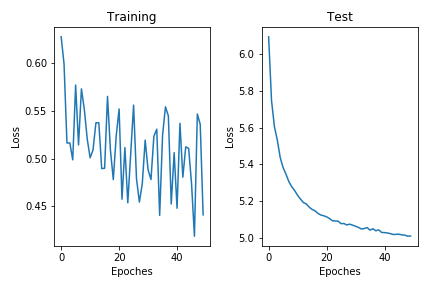
\includegraphics[width=.9\textwidth]{figures/auto_encoder_de_evolution}
	\caption{Evolution of Train and Test loss.}
\end{figure}
\begin{figure}[!btp]
	\centering
	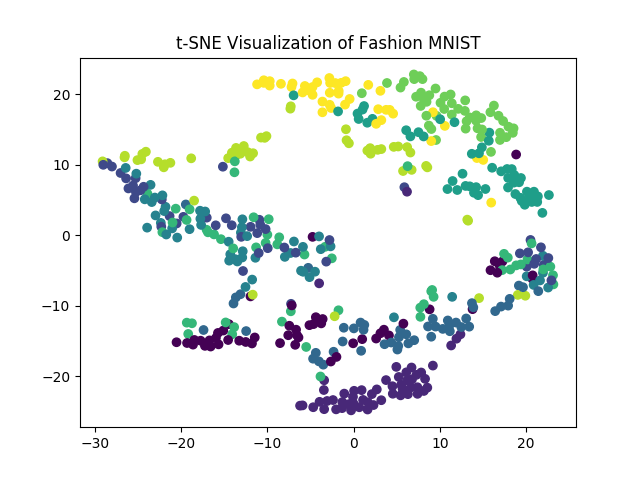
\includegraphics[width=.9\textwidth]{figures/t_sne_denois}
	\caption{TSNE representation.}
\end{figure}
\begin{figure}[!btp]
	\centering
	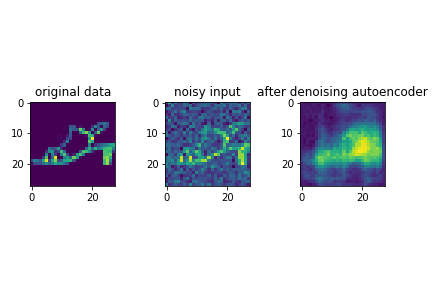
\includegraphics[width=.6\textwidth]{figures/save_ev_de_0}
	\caption{Original Image, noisy input and output.}
\end{figure}
\begin{figure}[!btp]
	\centering
	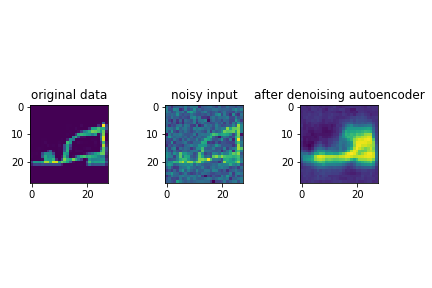
\includegraphics[width=.6\textwidth]{figures/save_ev_de_1}
	\caption{Original Image, noisy input and output.}
\end{figure}
\begin{figure}[!btp]
	\centering
	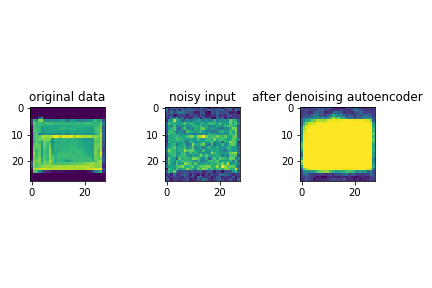
\includegraphics[width=.6\textwidth]{figures/save_ev_de_2}
	\caption{Original Image, noisy input and output.}
\end{figure}
\begin{figure}[!btp]
	\centering
	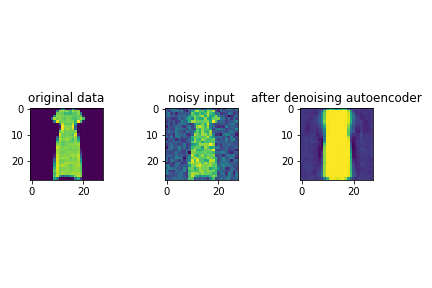
\includegraphics[width=.6\textwidth]{figures/save_ev_de_3}
	\caption{Original Image, noisy input and output.}
\end{figure}
\begin{figure}[!btp]
	\centering
	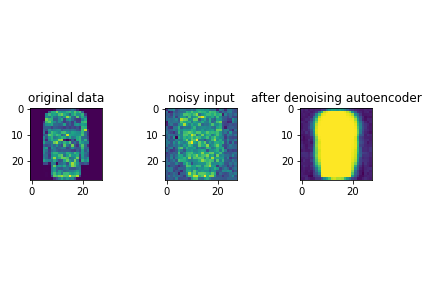
\includegraphics[width=.6\textwidth]{figures/save_ev_de_4}
	\caption{Original Image, noisy input and output.}
\end{figure}
\begin{figure}[!btp]
	\centering
	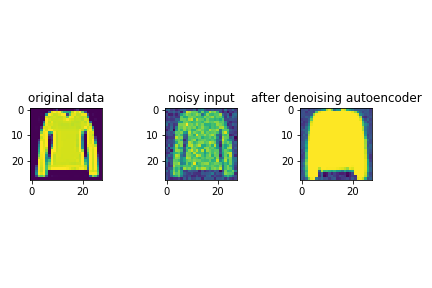
\includegraphics[width=.6\textwidth]{figures/save_ev_de_5}
	\caption{Original Image, noisy input and output.}
\end{figure}
\begin{figure}[!btp]
	\centering
	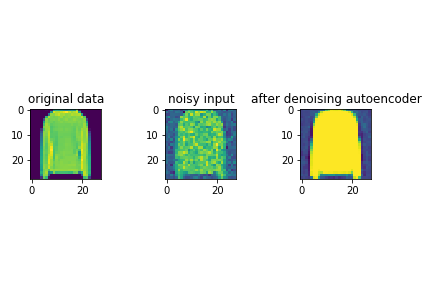
\includegraphics[width=.6\textwidth]{figures/save_ev_de_6}
	\caption{Original Image, noisy input and output.}
\end{figure}
\begin{figure}[!btp]
	\centering
	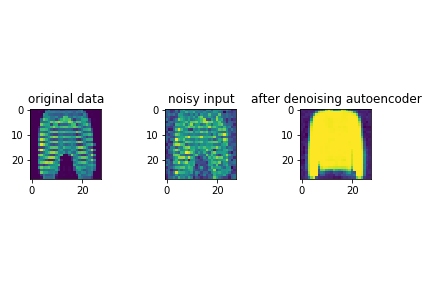
\includegraphics[width=.6\textwidth]{figures/save_ev_de_7}
	\caption{Original Image, noisy input and output.}
\end{figure}
\begin{figure}[!btp]
	\centering
	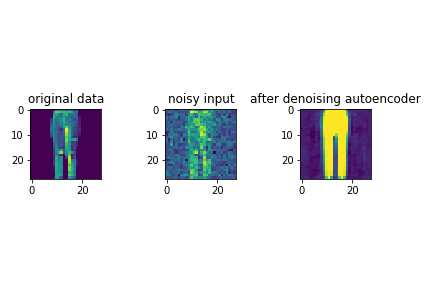
\includegraphics[width=.6\textwidth]{figures/save_ev_de_8}
	\caption{Original Image, noisy input and output.}
\end{figure}
\begin{figure}[!btp]
	\centering
	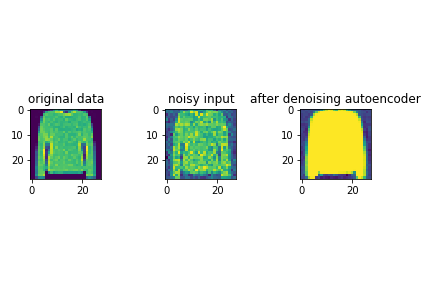
\includegraphics[width=.6\textwidth]{figures/save_ev_de_9}
	\caption{Original Image, noisy input and output.}
\end{figure}

\FloatBarrier

\newpage
\section{Appendix: Python Source Code}
\label{sec:app}

\subsection{Autoencoder}
\lstinputlisting[language=Python]{autoencoder.py}
\lstinputlisting[language=Python]{run_autoencoder.py}


\end{document}
